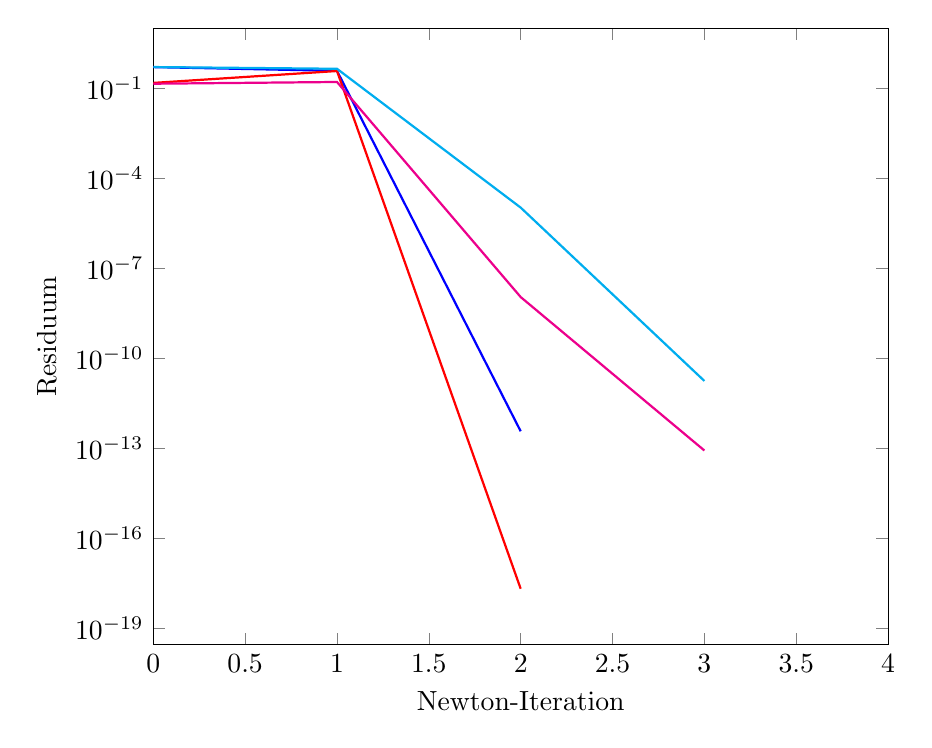
\begin{tikzpicture}[every plot/.append style={thick}] 
\begin{axis}[ 
label style={font=\normalsize}, 
xlabel={Newton-Iteration}, 
ylabel={Residuum}, 
xmin=0, xmax=4, 
ymode=log, 
ymin=0, ymax=10, 
width=0.9\textwidth, 
grid style=dashed, 
] 
\addplot[ 
color=blue, 
] 
coordinates { 
(0, 5.05e-01)(1, 3.79e-01)(2, 3.60e-13)}; 
\addplot[ 
color=red, 
] 
coordinates { 
(0, 1.50e-01)(1, 3.74e-01)(2, 2.01e-18)}; 
\addplot[ 
color=cyan, 
] 
coordinates { 
(0, 5.07e-01)(1, 4.44e-01)(2, 1.04e-05)(3, 1.72e-11)}; 
\addplot[ 
color=magenta, 
] 
coordinates { 
(0, 1.41e-01)(1, 1.61e-01)(2, 1.08e-08)(3, 8.23e-14)}; 
\end{axis} 
\end{tikzpicture} 
